\section{Sistemi lineari}
\todo{scrivi qualcosa qui}

\subsection{Sistemi dinamici}
Introduco alcuni concetti di base.

\begin{definition}
    Un insieme $\mathcal T \subseteq \R^+$ è detto \textbf{insieme del tempo}.
\end{definition}

\begin{definition}
    Un insieme $\Sigma \subseteq \R^{2n}$ è detto \textbf{spazio delle fasi}
    relativo a un sistema fisico quando i vettori
    $\b x \in \Sigma$ rappresentano tutti gli stati possibili
    del sistema, ovvero,
    tutte le $2n$-uple di coordinate e velocità generalizzate $(q_1, \dot q_1, \ldots, q_n, \dot q_n)$
    possibili per il sistema.
\end{definition}
La richiesta che lo spazio delle fasi abbia dimensione pari è dettata dal
fatto che, in generale, per definire lo stato di un sistema meccanico è
necessario conoscere sia il valore delle coordinate generalizzate
che delle rispettive velocità generalizzate associate.
È possibile definire uno spazio delle fasi che abbia dimensione dispari
oppure che sia un insieme dispcreto, ma ciò non è utile per quanto riguarda
questo testo. \todo{magari qui ci sta cit al turchetti che parla di questa roba all'inizio}

\begin{definition}
    Sia $t \in \mathcal T$ insieme del tempo, $\Sigma$ spazio delle fasi di un sistema e siano $\b x_0, \b x(t) \in \Sigma$.
    L'applicazione: \\
    \begin{equation*}
        \begin{array}{cccc}%
            \phi: &\mathcal T \times \Sigma &\to &\Sigma \\
            &\phi^t(\b x_0) &\mapsto &\b x(t)
        \end{array}%
    \end{equation*}
    è detta \textbf{flusso di fase} se e solo se rispetta le seguenti proprietà:
    \begin{itemize}
        \item \textbf{Identità:} $\phi^0(\b x_0) = \b x_0$.
        \item \textbf{Composizione:} $\phi^t \circ \phi^s = \phi^{t+s}$.
        \raggedright
        \item \textbf{Conservazione della misura:} esiste una misura $\mu$ di $\Sigma$ %
        conservata $\int_A \det J_\phi \ d\mu~=~\int_{\phi^t(A)} d\mu$.
    \end{itemize}
\end{definition}

Ora uso le definizioni appena enunciate per introdurre il concetto di
\emph{sistema dinamico}.

\begin{definition}
    La tripla $(\Sigma, \mathcal T, \phi)$ in cui:
    \begin{itemize}
        \item $\Sigma$ è uno spazio delle fasi%
        \item $\mathcal T$ è un insieme del tempo%
        \item $\phi$ è un flusso di fase%
    \end{itemize}
    è detta \textbf{sistema dinamico}.
    \label{def:sistema-dinamico}
\end{definition}

A seconda di come è costruito il flusso di fase, un sistema dinamico
può essere categorizzato come \emph{lineare} o \emph{non lineare}.
Inoltre, a seconda della scelta di $\mathcal T$, il sistema è detto
\emph{a tempo continuo} oppure \emph{a tempo discreto}.

L'esempio \ref{ex:semaforo} mostra come è possibile costruire
il più semplice sistema dinamico.

\begin{example}
    \label{ex:semaforo}
    Voglio descrivere il comportamento di un semaforo stradale.
    Il semaforo può essere o verde o rosso e cambia colore a intervalli regolari.
    Posso definire lo spazio delle fasi del sistema come:
    \begin{equation*}
        \Sigma := \{\text{Verde}, \text{Rosso} \}.
    \end{equation*}
    Il tempo è discreto: $\mathcal T = \Z^+$ e definisco il flusso di fase $\phi$:
    \begin{equation*}
        \phi^t(\text Rosso) = \left\{
        \begin{array}{lrl}
            Verde &$t$ &dispari\\
            Rosso &$t$ &pari
        \end{array}
        \right.
    \end{equation*}
    \begin{equation*}
        \phi^t(\text Verde) = \left\{
        \begin{array}{lrl}
            Rosso &$t$ &dispari\\
            Verde &$t$ &pari
        \end{array}
        \right.
        .
    \end{equation*}
    La tripla $(\Sigma, \mathcal T, \phi)$ è un \emph{sistema dinamico}.
    Il sistema è illustrato in figura \ref{fig:esempio-semaforo}.
    \begin{figure}[H]
        \centering
        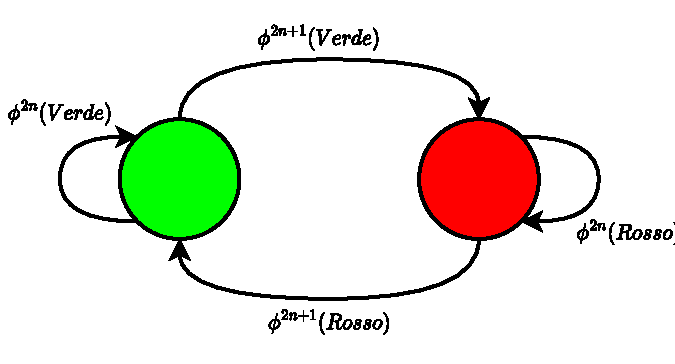
\includegraphics[width=0.5\textwidth]{assets/ex-semaforo}
        \caption[Semaforo]{Esempio di un semaforo come sistema dinamico.
        Gli stati possibili del sistema sono i due colori e il flusso di fase
        regola l'evoluzione temporale del sistema.}
        \label{fig:esempio-semaforo}
    \end{figure}
\end{example}


In generale, dalla osservazione di un sistema fisico si riesce a costruire un campo vettoriale
di equazioni differenziali che ne descrive il moto:
\begin{equation*}
    \dot {\b x} (t) = \b a(\b x).
\end{equation*}
È naturale quindi chiedersi \emph{come e se} sia possibile ricavare il flusso di fase partendo
dal campo vettoriale (e viceversa).
Si può dimostrare \todo{devo mettere la dimostrazione?} che vale la relazione~\eqref{eq:campo-vettoriale},
che mette quindi in relazione ogni sistema di equazioni differenziali con un rispettivo sistema dinamico.
\begin{equation}
    \b a (\b x) = \left.\frac d {dt} \right| _{t=0} \phi^t (\b x_0).
    \label{eq:campo-vettoriale}
\end{equation}

La \eqref{eq:campo-vettoriale} è, in generale, impossibile da integrare analiticamente.
Tuttavia, per i sistemi lineari, esiste una soluzione in forma chiusa.
Questa proprietà dei sistemi lineari è molto utile, dato che permette di trasformare un sistema
da tempo continuo a tempo discreto e viceversa.
Mostrerò come nel paragrafo seguente.
\todo{eventualmente, posso fare un esempio di campo vettoriale mostrando il flow delle fasi...
Non so se serve, per ora non lo faccio.}


\subsection{Equazioni differenziali lineari}
\label{subsec:equazioni-differenziali-lineari}
Introduco la definizione di \emph{equazione differenziale lineare}.
\begin{definition}
    Sia $\b x = \b x(t) \in \R^n$, $A \in \M_{2\times 2}(\R)$, ovvero, lo spazio vettoriale delle
    matrici $n \times n$ a coefficienti reali. Un'equazione nella forma
    \begin{equation}
        \dot{\b x} = A \b x
        \label{eq:sistema-lineare}
    \end{equation}
    è detta \textbf{equazione differenziale} (o sistema di equazioni differenziali) \textbf{lineare omogenea di \rom{1} ordine.}
    \label{def:sistema-lineare}
\end{definition}
\todo {glossario e small caps}

Per le equazioni del tipo~\eqref{eq:sistema-lineare} esiste una soluzione analitica
\begin{equation}
    \b x(t) = e^{\b A t} \b x(0),
    \label{eq:soluzione-lineare}
\end{equation}
dove l'esponenziale di matrice è definito da
\begin{equation*}
    e^{A} = \sum_{k=0}^{+\infty} \frac{A^k}{k!}.
    %\label{eq:exp-matrice}
\end{equation*}

Per dimostrare che la~\eqref{eq:soluzione-lineare} è soluzione è
sufficiente sostituirla nella~\eqref{eq:sistema-lineare} e verificare che
si ottiene un'identità.
Inoltre, il teorema~\ref{thm:esistenza-unicità} garantisce che,
fissate le condizioni iniziali, la
soluzione è unica.

\begin{thm}[Esistenza e unicità della soluzione]
    Siano:
    \begin{itemize}
        \item $Y \subseteq \R^n$ spazio di Banach.%
        \item $I \subseteq R$ intervallo.%
        \item $\b a(t, \b y) : I \times Y \to Y$ continua rispetto a $t$ e lipshitziana rispetto a $\b y$.%
        \item $(t_0, \b y_0) \in I \times Y$.
    \end{itemize}
    Allora il problema di Cauchy
    \begin{equation*}
        \left\{
            \begin{array}{ll}
                \dot{\b y}(t) &= \b a(t, \b y (t)) \\
                \b y (t_0) &= \b y_0
            \end{array}
        \right.
       %\label{eq:cauchy-problem}
    \end{equation*}
    ammette un'unica soluzione $\b \phi$ tale che $\dot {\b \phi}(t) = \b a(t, \b \phi(t))$
    identicamente in $I$ e $\b \phi(t_0) = \b y_0$.
    \label{thm:esistenza-unicità}
\end{thm}

La soluzione~\eqref{eq:soluzione-lineare}
corrisponde al flusso di fase associato al sistema dinamico che ha come campo vettoriale
associato $\b a(\b x) = A\b x$.
Infatti, considerando la proprietà~\eqref{eq:campo-vettoriale} e prendendo
$\phi^t(\b x) = e^{At} \b x$ trovo
\begin{equation*}
        \left. \frac d{dt} \right|_{t=0} e^{At} \b x_0 = A \b x.
\end{equation*}

\todo {Qui posso dire qualcosa riguardo alla possibilità di calcolare
esponenziale di matrici per sistemi diagonalizzabili.}

Questa possibilità di ricavare il flusso di fase partendo dal campo vettoriale per
sistemi lineari è utile, in quanto permette di passare da un sistema a tempo continuo
a un sistema a tempo discreto.
Fissato un intervallo di tempo $\Delta t$, le equazioni~\eqref{eq:mapping-sistema} descrivono lo stesso sistema fisico usando
rispettivamente un insieme del tempo discreto e uno continuo.

\begin{equation}
    \begin{array}{l}
        \mathcal T = \{0, \Delta t, 2\Delta t, \ldots\}, \\
        \b x_{k+1} = e^{A \Delta t} \b x_k
    \end{array}
        \leftrightarrow
    \begin{array}{l}
        \mathcal T = [0, +\infty [, \\
        \dot{\b x} = A \b x,
    \end{array}
    \label{eq:mapping-sistema}
\end{equation}
con $\b x_{k+1} = \b x(k\Delta t)$ e $\b x = \b x(t)$.

Tutte queste considerazioni possono essere estese anche ai sistemi lineari
\emph{non omogenei}.


\begin{definition}
    Sia $\b x = \b x(t) \in \R^n$, $A \in \M_{n\times n}(\R)$, $B \in \M_{n\times m}(\R)$ e $\b u = \b u(t) \in C^0(\R, \R^n)$.
    Un'equazione nella forma
    \begin{equation}
        \dot{\b x} = A \b x + B \b u
        \label{eq:sistema-lineare-non-omogeneo}
    \end{equation}
    è detta \textbf{equazione differenziale} (o sistema di equazioni differenziali) \textbf{lineare non omogenea di \rom{1} ordine.}
    \label{def:sistema-lineare-non-omogeneo}
\end{definition}

La soluzione per equazioni del tipo~\eqref{eq:sistema-lineare-non-omogeneo} è data da
\begin{equation}
    \b x(t) = e^{At} \b x(0) + \int_{0}^{t} e^{A(t-s)} B \b u(s) \ ds.
    \label{eq:soluzione-lineare-non-omogeneo}
\end{equation}
Se si impone che $\b u = \b u_k$ sia costante nell'intervallo di tempo $[k \Delta t, (k + 1)\Delta t]$,
la soluzione prende la forma
\begin{equation*}
    \b x_{k+1} = A_d \b x_k + B_d \b u_k
\end{equation*}
analoga alla~\eqref{eq:mapping-sistema}, con
\begin{align*}
    A_d &= e^{A\Delta t} \\
    B_d &= \int_0^{\Delta t}e^{As} B\ ds.
\end{align*}
%todo cite PII: S0098-1354(99)00007-1

Nel corso di questo testo, userò il termine generale \emph{"sistema"} per indicare
un sistema dinamico a cui è associata un equazione differenziale. Assumerò che le variabili
coinvolte siano ristrette agli spazi definiti dal sistema dinamico.


\subsection{Linearizzazione di un sistema non lineare}
\label{subsec:linearizzazione}
Considero un sistema dinamico caratterizzato da un campo vettoriale del tipo
\begin{equation}
    \dot {\b x} = \b a(\b x, \b u),\ \text{con}\ \b x = \b x (t)\ \text e \ \b u = \b u (t).
    \label{eq:sistema-non-lineare}
\end{equation}
È possibile linearizzare la dinamica del sistema~\eqref{eq:sistema-non-lineare} in un intorno di un punto fisso
$(\bar{\b x}, \bar{\b u})$ (che, per semplicità, prendo uguale a $(\b 0, \b 0)$) espandendo
in serie di Taylor:
\begin{equation}
    \b a(\b x, \b u) \approx \b a(\b 0, \b 0) +
    \left.\frac{d \b a}{d \b x}\right|_{(\b 0, \b 0)} \b x +
    \left.\frac{d \b a}{d \b u}\right|_{(\b 0, \b 0)} \b u + \mathcal O(\norm{(\b x, \b u)}^2).
    \label{eq:formula-linearizzazione}
\end{equation}
$\b a(\b 0, \b 0)$ si annulla (perchè corrisponde a un punto fisso) e posso riscrivere
gli altri due termini in forma matriciale, riconducendomi alla forma~\eqref{def:sistema-lineare-non-omogeneo}
della definizione~\ref{def:sistema-lineare-non-omogeneo}.

Per chiarezza, le matrici $A$ e $B$ sono definite dalla~\eqref{eq:matrici-A-B}.
\begin{equation}
    A_{ij} = \frac{df_i}{dx_j},\ B_{ij} = \frac{df_i}{du_j}.
    \label{eq:matrici-A-B}
\end{equation}
\todo{controlla questa cosa qui perchè sono 99\% sicuro che sia giusta ma non ho controllato.}

\subsection{Comportamento asintotico delle soluzioni}
\label{subsec:comportamento-asintotico}
Le soluzioni di un sistema lineare omogeneo possono avere solo uno di tre comportamenti asintotici:
\begin{itemize}
    \item convergere a zero,
    \item divergere,
    \item oscillare attorno a zero.
\end{itemize}
Il comportamento è determinato interamente dagli autovalori della matrice $A$ che definisce il
sistema, secondo la~\eqref{eq:sistema-lineare}.
Le condizioni sufficienti per avere un certo comportamento sono riassunte nella proposizione~\ref{prop:comportamento-asintotico}.
\begin{prop}
    Sia $A$ la matrice associata a un sistema di equazioni differenziali omogeneo,
    definita secondo la definizione~\ref{def:sistema-lineare}.
    Se $A$ è diagonalizzabile, il comportamento asintotico delle soluzioni è interamente
    determinato dagli autovalori di $A$:
    \begin{itemize}
        \item Se tutti gli autovalori hanno parte reale \textbf{neativa}, allora $\norm{\b x(t)} \to 0$ per $t \to +\infty$.%
        \item Se almeno un autovalore hanno parte reale \textbf{positiva}, allora $\norm{\b x(t)} \to 0$ per $t \to +\infty$.%
        \item Se tutti gli autovalori hanno parte reale \textbf{nulla}, allora le soluzioni sono periodiche.
    \end{itemize}
    \label{prop:comportamento-asintotico}
\end{prop}

\emph{Dimostrazione}.
Lavoro nella base in cui $A$ è diagonale.
In questa base, l'equazione differenziale diventa
\begin{equation}
    \dot{\b z} = \Lambda \b z,
    \label{eq:diagonale}
\end{equation}
dove $\Lambda$ è la matrice che ha sulla diagonale
gli autovalori di $A$ e $\b z, \dot{\b z}$ sono i vettori $\b x, \dot{\b x}$ rappresentati secondo la nuova base.
Sia $T$ la matrice di cambio base, allora $\Lambda$ è data da \todo{la fioresi la chiama così ma dovrei scrivere la definizione...}.
\begin{equation*}
    \Lambda = T^{-1} A T,
\end{equation*}
$\b z$ è dato da
\begin{equation*}
    \b z = T^{-1} \b x
\end{equation*}
e, dato che $A$ non dipende dal tempo, $\dot{\b z}$ è dato da
\begin{equation*}
    \dot{\b z} = T^{-1} \dot{\b x}.
\end{equation*}
Riscrivo la~\eqref{eq:diagonale} in notazione indiciale.
Se $\lambda_i, i = 0, \ldots, n$ sono gli elementi sulla diagonale di $\Lambda$, vale:
\begin{equation*}
    \dot z_i = \delta_{ij} \lambda_i z_j.
\end{equation*}
Mi sono quindi ricondotto a $n$ equazioni differenziali omogenee di \rom{1} ordine, che
hanno come soluzione
\begin{equation*}
    z_i(t) = e^{\lambda_i t},
\end{equation*}
dove ho preso $z_i(0) = 0$.
Gli autovalori sono numeri complessi $\lambda_j = a_j + i b_j$, quindi le soluzioni
sono date dalla~\eqref{eq:soluzioni-complesse}.
\begin{equation}
    e^{\lambda_j t} = e^{a_j t}\left(\cos{b_j t} + i\sin{b_j t} \right).
\label{eq:soluzioni-complesse}
\end{equation}
La dimostrazione termina calcolando il limite per $t \to +\infty$
della~\eqref{eq:soluzioni-complesse} nei tre casi considerati.
\hfill \qedsymbol \paragraph{}

Per i sistemi a tempo discreto si ottengono condizioni diverse sugli autovalori
che riporto nella proposizione~\ref{prop:comportamento-asintotico-discreto}, senza
dimostrazione.
\begin{prop}
    Sia $A_d = e^{A\Delta t}$ la matrice associata a un sistema di equazioni differenziali omogeneo
    a tempo discreto:
    \begin{equation*}
        \b x_{k+1} = A_d \b x_k.
    \end{equation*}
    Se $A_d$ è diagonalizzabile, il comportamento asintotico delle soluzioni è interamente
    determinato dagli autovalori di $A_d$:
    \begin{itemize}
        \item Se tutti gli autovalori hanno modulo \textbf{minore di $1$}, allora $\norm{\b x_k} \to 0$ per $k \to +\infty$.%
        \item Se almeno un autovalore ha modulo \textbf{maggiore di $1$}, allora $\norm{\b x_k} \to 0$ per $k \to +\infty$.%
        \item Se tutti gli autovalori hanno \textbf{modulo uguale a $1$}, allora le soluzioni sono periodiche.
    \end{itemize}
    \label{prop:comportamento-asintotico-discreto}
\end{prop}